\lstdefinestyle{mystyle}{
    backgroundcolor=\color{myyellow},
    basicstyle=\ttfamily\small,
    breaklines=true,
    frame=single,
    language=XML
}

\chapter{State-of-the-Art Analysis} \label{ch:state-of-the-ArtAnalysis}
The following chapter constitutes an in-depth exploration of current technologies and methodologies within the automotive industry, with a specific focus on the complexity of vehicular software development. Firstly, the current automotive landscape will be examined, providing a detailed insight into challenges associated with software development in vehicles.

Subsequently, through meticulous analysis of scientific publications, technical reports, and practical implementations, the chapter delves into the radical transformation of the automotive sector facilitated by the concept of Software Defined Vehicle (SDV). This technology, crucial for technological progress and vehicular safety, will be explored from various perspectives. Particularly, the synergy between Cloud, software, and hardware will be investigated, highlighting solutions proposed by major industry players and analyzing their applications, benefits, and limitations.

The objective is to offer a comprehensive overview of current dynamics, emphasizing the pivotal role of SDV in the evolution of the automotive industry.

\section{Current Automotive Software Development}

In the past, the automotive industry advanced primarily through the development of technologies in mechanical engineering, focusing on perfecting combustion engines. Nowadays, the paradigm has radically changed due to multiple factors, including electrification, automation, shared mobility, and connected mobility.

Software technology development in the automotive field can be metaphorically compared to what has happened in smartphone development, as highlighted in the manifesto document regarding Bosch's Software Defined Vehicle (SDV) \cite{SDVBoshMobility}.

The ultimate goal is to achieve simple and user-friendly devices that fully meet the user's needs. Currently, many customers express dissatisfaction because their cars do not offer the same functionality and ease of use common in smartphones. Many ask: Why can't my \$50,000 car perform the same tasks as my \$300 smartphone?

A key difference between the automotive and smartphone industries is the level of complexity, which brings with it a number of issues.

\subsection{difficulties}
We can analyse in depth the problems of the current automotive software that is being developed via 4 main difficulties:

\begin{itemize}
    \item Specialized Hardware: Today's vehicles are still complex systems of systems. Each subsystem in a car, from brakes to transmission, is a complex entity, supplied by a different manufacturer and integrated with a unique software architecture. The level of complexity and the need for seamless interoperability between systems far exceeds that of today's smartphones.
    \item Time: The software production pipeline involves many development and testing steps with a not inconsiderable amount of time spent on each one. This is greatly increased by the presence of different components, so development time must be considered for each different unit of the system.
    \item Cost: The complexity of the software systems in vehicles entails very high costs, aggravated by the fact that the test phase is often carried out directly on the boards (for hardware requirements), which means a much longer production process, especially in the event of errors.
    
    \begin{figure}[h]  % 'h' significa che la figura viene posizionata qui
        \centering
        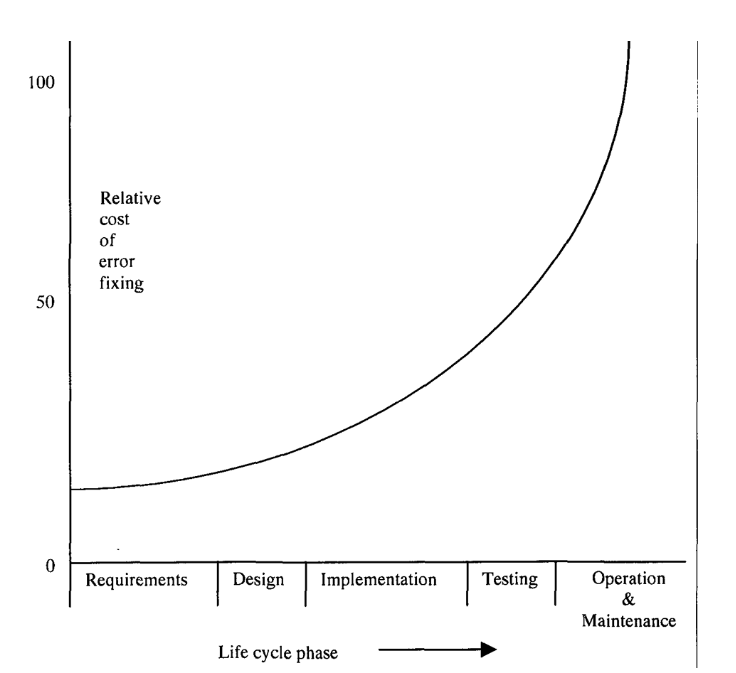
\includegraphics[width=0.9\textwidth]{images/costs_of_errors_correction_in_software_development.png}  % Sostituisci 'nome_immagine' con il nome del tuo file immagine e l'estensione
        \caption{Cost of fixing errors increases in later phases of the life cycle \cite{CostsOfSoftwareDeveloping}}
        \label{fig:WorldAutomobileProduction}
      \end{figure}

    \item Human Safety Security: Automotive embedded software must meet stringent reliability and security requirements, while delivering performance and a reasonable memory footprint. To develop automotive embedded software, you need the right tools that meet safety and security standards to evaluate, prototype and test your software.
\end{itemize}

What lessons can be drawn from the study of barriers that can be applied to the vehicle lifecycle? Historically, the vehicle lifecycle has been characterised by the simultaneous production and deployment of tightly integrated hardware and software. Once the vehicle was in the hands of the consumer, its characteristics remained largely unchanged until the end of its life. However, the SDV paradigm introduces the possibility of decoupling hardware and software release dates - a prerequisite for adopting a digital-first approach. This approach brings the design and virtual validation of the digital vehicle experience to the forefront of the lifecycle.

There is also a need to apply the digital-first concept, which means that new ideas for the vehicle experience are first explored in virtual environments to ensure early user feedback, long before any custom hardware needs to be developed or a physical test vehicle is available. Digital first is the application of design thinking and lean startup principles, originally rooted in internet culture, to the tangible realm of automotive development.
\section{Introduction to Software Defined Vehicle}
%“Automakers and their suppliers need to continuously review and improve the testing approach in design and development, as well as look for new tools that automate and increase test coverage of their products,” Giallorenzo explained. “Cloud emulation is a major innovation that is coming to the industry to facilitate development and testing. Historically, testing of embedded software solutions has been hindered by the lack of chipsets and hardware, which is required to properly test complete hardware-plus-software solutions. This was particularly painful during the recent COVID-induced supply chain crunch."

%Automotive engineering has traditionally focused on physical functionality, from early electronic features (such as airbags, vehicle stabilization, and braking systems) to modern driver assistance systems or even automated driving. The new, digital experience is driven by software-enabled features, and the focus is on improving the experience of using the vehicle or even providing value-added digital features like usage-based insurance or automated payment of parking fees. Figure 1-4 shows some of these differences.
\subsection{Benefits}
\subsection{Enablers}
